\documentclass[12pt]{article}

% ============================================================================
% PACKAGES
% ============================================================================
\usepackage[utf8]{inputenc}
\usepackage[T1]{fontenc}
\usepackage{amsmath,amssymb,amsthm}
\usepackage{mathtools}
\usepackage[margin=1in]{geometry}
\usepackage{hyperref}
\usepackage{booktabs}
\usepackage{graphicx}
\usepackage{xcolor}
\usepackage{fancyvrb}
\usepackage{tikz}
\usepackage{float}
\usetikzlibrary{arrows,shapes,positioning,calc,decorations.pathreplacing}

% Braket notation (manual)
\newcommand{\ket}[1]{|#1\rangle}
\newcommand{\bra}[1]{\langle#1|}
\newcommand{\braket}[2]{\langle#1|#2\rangle}

% ============================================================================
% THEOREM ENVIRONMENTS
% ============================================================================
\theoremstyle{plain}
\newtheorem{theorem}{Theorem}[section]
\newtheorem{proposition}[theorem]{Proposition}
\newtheorem{corollary}[theorem]{Corollary}
\newtheorem{lemma}[theorem]{Lemma}

\theoremstyle{definition}
\newtheorem{definition}[theorem]{Definition}
\newtheorem{principle}[theorem]{Operating Principle}

% ============================================================================
% CUSTOM COMMANDS
% ============================================================================
\newcommand{\phival}{\varphi}
\newcommand{\Tphi}{T_\varphi}
\newcommand{\Egap}{E_{\text{gap}}}
\newcommand{\Coh}{\mathcal{C}}
\newcommand{\R}{\mathbb{R}}
\newcommand{\C}{\mathbb{C}}
\newcommand{\Tr}{\mathrm{Tr}}
\newcommand{\kB}{k_{\text{B}}}

% ============================================================================
% TITLE
% ============================================================================
\title{
\textbf{UNITED STATES PATENT APPLICATION}\\[1em]
\Large Golden Ratio Critical Temperature for\\
Quantum Coherence Optimization
}

\author{
\textbf{Inventor:} Jonathan Washburn\\
Recognition Science Research Institute\\
\texttt{jonathan@recognitionscience.org}
}

\date{Filing Date: December 31, 2025}

\begin{document}

\maketitle
\thispagestyle{empty}

% ============================================================================
% HEADER INFORMATION
% ============================================================================
\begin{center}
\begin{tabular}{ll}
\toprule
\textbf{Application Number:} & [To be assigned] \\
\textbf{Filing Date:} & December 31, 2025 \\
\textbf{Inventor:} & Jonathan Washburn \\
\textbf{Assignee:} & Recognition Science Research Institute \\
\textbf{Classification:} & G06N 10/40 (Quantum Coherence); H01L 39/00 \\
\bottomrule
\end{tabular}
\end{center}

\vspace{2em}

% ============================================================================
% ABSTRACT
% ============================================================================
\begin{abstract}
A method and system for optimizing quantum coherence using golden ratio-derived temperature thresholds and coherence order parameters. The invention establishes that the critical temperature for coherent quantum operation is $\Tphi = 1/\ln\phival \approx 2.078$ (in dimensionless units), where $\phival = (1+\sqrt{5})/2$ is the golden ratio. For a quantum system with energy gap $\Egap$, coherent operation requires temperature $T < \Tphi \cdot \Egap / \kB$. The coherence order parameter $\Coh$ provides real-time monitoring of quantum coherence, with $\Coh \geq 1$ indicating coherent operation and $\Coh < 1$ indicating decoherence onset. The invention provides: (1) a principled operating temperature bound for quantum devices; (2) golden ratio-based coherence monitoring thresholds; (3) adaptive cooling protocols maintaining $T/\Egap < \Tphi$; (4) phase transition detection at the $\Tphi$ boundary. Applications include superconducting qubits, quantum sensors, atomic clocks, quantum memories, and coherent optical systems.

\vspace{0.5em}
\noindent\textbf{Keywords:} quantum coherence, decoherence, critical temperature, golden ratio, order parameter, quantum computing, quantum sensing
\end{abstract}

\newpage
\setcounter{page}{1}

% ============================================================================
% FIELD OF THE INVENTION
% ============================================================================
\section{Field of the Invention}

The present invention relates generally to quantum systems and quantum information processing, and more particularly to methods for optimizing and monitoring quantum coherence using golden ratio-derived temperature thresholds and order parameters.

% ============================================================================
% BACKGROUND OF THE INVENTION
% ============================================================================
\section{Background of the Invention}

\subsection{Technical Background}

Quantum coherence---the ability of a quantum system to exist in superposition states---is essential for quantum computing, quantum sensing, and quantum communication. Coherence is fragile and destroyed by thermal fluctuations, environmental noise, and measurement.

\subsubsection{Decoherence Mechanisms}

\begin{itemize}
    \item \textbf{Thermal decoherence:} Thermal energy $\kB T$ excites transitions that destroy superpositions when $\kB T \gtrsim \Egap$.
    
    \item \textbf{Dephasing:} Random phase kicks from environmental fluctuations.
    
    \item \textbf{Relaxation:} Energy exchange with the thermal bath.
    
    \item \textbf{Measurement-induced:} Projective collapse from environmental coupling.
\end{itemize}

\subsubsection{Temperature Requirements}

For coherent quantum operation, systems typically require:
\begin{equation}
\kB T \ll \Egap
\end{equation}
where $\Egap$ is the relevant energy gap (e.g., qubit splitting, transition energy).

Current practice uses heuristic temperature bounds:
\begin{itemize}
    \item Superconducting qubits: $T < 20$ mK for $\Egap \sim 5$ GHz
    \item Trapped ions: Laser cooling to $\mu$K range
    \item NV centers: Often room temperature (large gap)
\end{itemize}

\subsubsection{Coherence Characterization}

Coherence is typically characterized by:
\begin{itemize}
    \item $T_1$: Relaxation time (energy decay)
    \item $T_2$: Dephasing time (phase coherence)
    \item $T_2^*$: Inhomogeneous dephasing time
\end{itemize}

These times depend on temperature, but the precise relationship lacks a universal framework.

\subsection{Limitations of Prior Art}

\begin{enumerate}
    \item \textbf{No Universal Temperature Criterion:} The condition ``$\kB T \ll \Egap$'' is imprecise; ``$\ll$'' varies from $10\times$ to $100\times$ in practice.
    
    \item \textbf{Empirical Coherence Metrics:} $T_1$, $T_2$ are measured quantities without principled thresholds for ``sufficient'' coherence.
    
    \item \textbf{System-Specific Optimization:} Each quantum platform develops independent thermal engineering, with no unifying principle.
    
    \item \textbf{No Order Parameter:} Unlike phase transitions in statistical mechanics, quantum coherence lacks a standard order parameter.
\end{enumerate}

\subsection{References}

\begin{itemize}
    \item Zurek, W. H. (2003). ``Decoherence, einselection, and the quantum origins of the classical.'' \textit{Reviews of Modern Physics}, 75(3), 715.
    \item Schlosshauer, M. (2007). \textit{Decoherence and the Quantum-to-Classical Transition}. Springer.
    \item Krantz, P., et al. (2019). ``A quantum engineer's guide to superconducting qubits.'' \textit{Applied Physics Reviews}, 6(2), 021318.
    \item Degen, C. L., et al. (2017). ``Quantum sensing.'' \textit{Reviews of Modern Physics}, 89(3), 035002.
\end{itemize}

% ============================================================================
% SUMMARY OF THE INVENTION
% ============================================================================
\section{Summary of the Invention}

The present invention provides a universal framework for quantum coherence optimization based on the golden ratio critical temperature $\Tphi$ and coherence order parameter $\Coh$.

\subsection{Golden Ratio Critical Temperature}

The critical temperature for the coherence-decoherence transition is:
\begin{equation}
\boxed{\Tphi = \frac{1}{\ln\phival} \approx 2.078}
\end{equation}
where $\phival = (1+\sqrt{5})/2$ is the golden ratio.

In physical units, coherent operation requires:
\begin{equation}
\boxed{T < \frac{\Tphi \cdot \Egap}{\kB} = \frac{\Egap}{\kB \ln\phival}}
\end{equation}

\textbf{Interpretation:} The dimensionless ratio $\kB T / \Egap$ must be less than $\Tphi \approx 2.078$ for coherent operation.

\subsection{Coherence Order Parameter}

The coherence order parameter $\Coh$ quantifies the degree of quantum coherence:
\begin{equation}
\boxed{\Coh = \frac{\Egap}{\kB T \cdot \ln\phival} = \frac{\Tphi}{\kB T / \Egap}}
\end{equation}

Phase classification:
\begin{itemize}
    \item $\Coh > 1$: Coherent phase (quantum behavior dominant)
    \item $\Coh = 1$: Critical point (coherence boundary)
    \item $\Coh < 1$: Decoherent phase (classical behavior dominant)
\end{itemize}

\subsection{Theoretical Foundation}

The $\Tphi$ threshold emerges from Recognition Science:

\begin{enumerate}
    \item \textbf{Golden Ratio Boltzmann Factor:} At temperature $\Tphi$, the Boltzmann factor for unit energy is exactly $1/\phival$:
    \begin{equation}
    \exp\left(-\frac{1}{\Tphi}\right) = \exp(-\ln\phival) = \frac{1}{\phival} \approx 0.618
    \end{equation}
    
    \item \textbf{Self-Similar Thermal Occupation:} The ratio of excited to ground state populations at $\Tphi$ satisfies the golden ratio proportion.
    
    \item \textbf{Coherence-Decoherence Phase Transition:} $\Tphi$ marks the boundary where thermal fluctuations begin to dominate quantum coherence.
\end{enumerate}

\subsection{Key Advantages}

\begin{enumerate}
    \item \textbf{Universal Criterion:} Single dimensionless threshold $\Tphi \approx 2.078$ applies across platforms
    \item \textbf{Precise Bound:} Replaces vague ``$\ll$'' with exact $< \Tphi$
    \item \textbf{Order Parameter:} $\Coh$ provides quantitative coherence monitoring
    \item \textbf{Predictive:} Enables a priori thermal design without empirical fitting
    \item \textbf{Phase Transition Framework:} Connects quantum coherence to statistical mechanics
\end{enumerate}

% ============================================================================
% BRIEF DESCRIPTION OF DRAWINGS
% ============================================================================
\section{Brief Description of Drawings}

\begin{description}
    \item[FIG. 1] Phase diagram showing coherent and decoherent regions separated by the $\Tphi$ boundary.
    
    \item[FIG. 2] Coherence order parameter $\Coh$ as a function of temperature for various energy gaps.
    
    \item[FIG. 3] Boltzmann factor $\exp(-\Egap/\kB T)$ showing the golden ratio value at $T = \Tphi \cdot \Egap/\kB$.
    
    \item[FIG. 4] Operating temperature requirements for different quantum platforms.
    
    \item[FIG. 5] Flowchart for coherence-optimized thermal control system.
    
    \item[FIG. 6] Real-time coherence monitoring system with $\Coh$ feedback.
    
    \item[FIG. 7] Comparison of coherence times for $\Coh > 1$ vs.\ $\Coh < 1$ operation.
    
    \item[FIG. 8] Block diagram of quantum processor with golden ratio thermal management.
\end{description}

% ============================================================================
% DETAILED DESCRIPTION
% ============================================================================
\section{Detailed Description}

\subsection{Mathematical Foundation}

\subsubsection{The Golden Ratio}

The golden ratio is defined as:
\begin{equation}
\phival = \frac{1 + \sqrt{5}}{2} \approx 1.6180339887
\end{equation}

Key properties:
\begin{align}
\ln\phival &\approx 0.4812 \\
\frac{1}{\ln\phival} &= \Tphi \approx 2.078 \\
\exp(-\ln\phival) &= \frac{1}{\phival} \approx 0.618
\end{align}

\subsubsection{Derivation of Critical Temperature}

\begin{theorem}[Golden Ratio Critical Temperature]
The critical temperature for quantum coherence is $\Tphi = 1/\ln\phival$, at which the thermal occupation ratio equals the golden ratio complement.
\end{theorem}

\begin{proof}
Consider a two-level quantum system with ground state $\ket{0}$ and excited state $\ket{1}$ separated by energy $\Egap$. The thermal populations are:
\begin{align}
p_0 &= \frac{1}{1 + \exp(-\Egap/\kB T)} \\
p_1 &= \frac{\exp(-\Egap/\kB T)}{1 + \exp(-\Egap/\kB T)}
\end{align}

Define the dimensionless temperature $\tau = \kB T / \Egap$. The population ratio is:
\begin{equation}
\frac{p_1}{p_0} = \exp\left(-\frac{1}{\tau}\right)
\end{equation}

At the golden ratio critical point, we require:
\begin{equation}
\frac{p_1}{p_0} = \frac{1}{\phival}
\end{equation}

This gives:
\begin{equation}
\exp\left(-\frac{1}{\tau_c}\right) = \frac{1}{\phival} \implies \frac{1}{\tau_c} = \ln\phival \implies \tau_c = \frac{1}{\ln\phival} = \Tphi
\end{equation}

In physical units: $T_c = \Tphi \cdot \Egap / \kB \approx 2.078 \cdot \Egap / \kB$.
\end{proof}

\subsubsection{Coherence Order Parameter}

\begin{definition}[Coherence Order Parameter]
The coherence order parameter for a quantum system is:
\begin{equation}
\Coh = \frac{\Egap}{\kB T \cdot \ln\phival} = \frac{\Tphi}{\tau}
\end{equation}
where $\tau = \kB T / \Egap$ is the dimensionless temperature.
\end{definition}

Properties:
\begin{enumerate}
    \item $\Coh \to \infty$ as $T \to 0$ (perfect coherence)
    \item $\Coh = 1$ at $T = T_c$ (critical point)
    \item $\Coh \to 0$ as $T \to \infty$ (complete decoherence)
\end{enumerate}

\begin{theorem}[Coherence Phase Transition]
The coherence order parameter $\Coh$ exhibits a phase transition at $\Coh = 1$:
\begin{itemize}
    \item For $\Coh > 1$ (coherent phase): Quantum superpositions are thermally stable
    \item For $\Coh < 1$ (decoherent phase): Thermal fluctuations destroy coherence
\end{itemize}
\end{theorem}

\subsubsection{Relationship to Coherence Times}

The coherence times scale with the order parameter:
\begin{align}
T_1 &\propto \exp(\Coh) \cdot T_1^{(0)} \\
T_2 &\propto \Coh \cdot T_2^{(0)}
\end{align}
where $T_1^{(0)}$, $T_2^{(0)}$ are intrinsic (zero-temperature) limits.

For $\Coh \gg 1$: Coherence times approach intrinsic limits.\\
For $\Coh \lesssim 1$: Thermal decoherence dominates.

% ----------------------------------------------------------------------------

\subsection{Operating Temperature Requirements}

\subsubsection{General Criterion}

For coherent operation, maintain:
\begin{equation}
T < T_{\max} = \frac{\Egap}{\kB \ln\phival} \approx \frac{2.078 \cdot \Egap}{\kB}
\end{equation}

With safety margin $\alpha$:
\begin{equation}
T_{\text{operating}} < \frac{T_{\max}}{\alpha} = \frac{\Egap}{\alpha \cdot \kB \ln\phival}
\end{equation}

Recommended: $\alpha = \phival$ (golden margin), giving:
\begin{equation}
T_{\text{operating}} < \frac{\Egap}{\phival \cdot \kB \ln\phival} \approx \frac{1.284 \cdot \Egap}{\kB}
\end{equation}

\subsubsection{Platform-Specific Requirements}

\begin{center}
\begin{tabular}{lccc}
\toprule
\textbf{Platform} & \textbf{$\Egap/h$} & \textbf{$T_c = \Tphi \Egap/\kB$} & \textbf{Typical $T_{\text{op}}$} \\
\midrule
Superconducting qubit & 5 GHz & 500 mK & 15 mK \\
Transmon & 6 GHz & 600 mK & 20 mK \\
Trapped ion & 10 THz & 1000 K & 1 mK \\
NV center & 3 GHz & 300 mK & 300 K$^*$ \\
Quantum dot & 1 meV & 24 K & 100 mK \\
\bottomrule
\end{tabular}
\end{center}

$^*$NV centers operate above $T_c$ for the primary transition but use alternative coherence mechanisms.

\subsubsection{Coherence Budget}

For a quantum algorithm requiring $N$ operations:
\begin{equation}
\Coh > \Coh_{\min} = \ln(N) / \ln\phival \approx 2.078 \ln(N)
\end{equation}

This ensures thermal errors remain negligible over the computation.

% ----------------------------------------------------------------------------

\subsection{Coherence Monitoring System}

\subsubsection{Real-Time $\Coh$ Measurement}

\begin{principle}[Coherence Monitoring]
Continuously monitor the coherence order parameter $\Coh$ and maintain $\Coh > 1$ (with margin) for coherent operation.
\end{principle}

Measurement approaches:
\begin{enumerate}
    \item \textbf{Temperature monitoring:} Measure $T$, compute $\Coh = \Tphi \cdot \Egap / (\kB T)$
    \item \textbf{Population measurement:} Measure $p_1/p_0$, compute $\Coh = -\ln(p_1/p_0) / \ln\phival$
    \item \textbf{Coherence tomography:} Measure off-diagonal density matrix elements
\end{enumerate}

\subsubsection{Feedback Control}

\begin{Verbatim}[frame=single,fontsize=\small]
COHERENCE FEEDBACK CONTROLLER

INPUT: Target coherence C_target, energy gap E_gap
OUTPUT: Temperature setpoint T_set

1. phi <- (1 + sqrt(5)) / 2
2. T_phi <- 1 / ln(phi)

3. LOOP:
4.     C_current <- measure_coherence()
5.     
6.     IF C_current < C_target:
7.         // Increase cooling
8.         T_set <- T_set * (1 - 1/phi)  // Reduce by 38.2%
9.     ELSE IF C_current > C_target * phi:
10.        // Reduce cooling (energy saving)
11.        T_set <- T_set * (1 + 1/phi^2)  // Increase by 38.2%
12.    
13.    apply_temperature(T_set)
14.    WAIT sampling_interval
\end{Verbatim}

\subsubsection{Alert Thresholds}

\begin{center}
\begin{tabular}{lcl}
\toprule
\textbf{$\Coh$ Range} & \textbf{Status} & \textbf{Action} \\
\midrule
$\Coh > \phival^2 \approx 2.62$ & Excellent & Nominal operation \\
$\phival < \Coh < \phival^2$ & Good & Monitor closely \\
$1 < \Coh < \phival$ & Warning & Increase cooling \\
$\Coh < 1$ & Critical & Emergency cooling / halt operations \\
\bottomrule
\end{tabular}
\end{center}

% ----------------------------------------------------------------------------

\subsection{Adaptive Cooling Protocol}

\subsubsection{$\phival$-Ladder Cooling}

For systems requiring staged cooling:

\begin{Verbatim}[frame=single,fontsize=\small]
PHI-LADDER COOLING PROTOCOL

INPUT: Initial temperature T_init, target coherence C_target
OUTPUT: Cooling schedule

1. phi <- (1 + sqrt(5)) / 2
2. T_phi <- 1 / ln(phi)

3. // Compute target temperature
4. T_target <- T_phi * E_gap / (k_B * C_target)

5. // Generate phi-ladder
6. T_current <- T_init
7. stage <- 0

8. WHILE T_current > T_target:
9.     T_next <- T_current / phi
10.    COOL from T_current to T_next
11.    WAIT for thermal equilibration
12.    stage <- stage + 1
13.    T_current <- T_next

14. STABILIZE at T_target
\end{Verbatim}

\subsubsection{Energy-Efficient Cooling}

The golden ratio provides optimal cooling efficiency:
\begin{equation}
\eta = \frac{\Delta \Coh}{\Delta E_{\text{cooling}}} \propto \frac{1}{\phival^k}
\end{equation}

Each $\phival$-step achieves:
\begin{itemize}
    \item Temperature reduction by factor $1/\phival \approx 0.618$
    \item Coherence increase by factor $\phival \approx 1.618$
    \item Cooling energy proportional to $\phival^{-1}$ of previous step
\end{itemize}

% ----------------------------------------------------------------------------

\subsection{Implementation}

\subsubsection{Python Implementation}

\begin{Verbatim}[frame=single,fontsize=\small]
"""
Golden Ratio Coherence Optimization
Patent Implementation
"""

import numpy as np
from typing import Tuple, Optional
from dataclasses import dataclass

# Physical constants
K_B = 1.380649e-23  # Boltzmann constant (J/K)
H = 6.62607015e-34  # Planck constant (J·s)

# Golden ratio constants
PHI = (1 + np.sqrt(5)) / 2          # ~1.618
T_PHI = 1 / np.log(PHI)             # ~2.078
LN_PHI = np.log(PHI)                # ~0.481


@dataclass
class CoherenceState:
    """State of coherence monitoring."""
    temperature: float      # Kelvin
    energy_gap: float       # Joules
    coherence: float        # Order parameter C
    phase: str              # 'coherent', 'critical', 'decoherent'


class GoldenRatioCoherenceOptimizer:
    """
    Coherence optimization using golden ratio critical temperature.
    
    Critical temperature: T_phi = 1/ln(phi) ~ 2.078 (dimensionless)
    Physical critical: T_c = T_phi * E_gap / k_B
    """
    
    def __init__(self, energy_gap_joules: float):
        """
        Initialize coherence optimizer.
        
        Parameters
        ----------
        energy_gap_joules : float
            Energy gap in Joules (or use from_frequency/from_ghz)
        """
        self.E_gap = energy_gap_joules
        self.T_critical = T_PHI * self.E_gap / K_B
    
    @classmethod
    def from_frequency(cls, freq_hz: float) -> 'GoldenRatioCoherenceOptimizer':
        """Create from transition frequency in Hz."""
        return cls(H * freq_hz)
    
    @classmethod
    def from_ghz(cls, freq_ghz: float) -> 'GoldenRatioCoherenceOptimizer':
        """Create from transition frequency in GHz."""
        return cls(H * freq_ghz * 1e9)
    
    @property
    def critical_temperature(self) -> float:
        """Critical temperature in Kelvin."""
        return self.T_critical
    
    def coherence_parameter(self, temperature: float) -> float:
        """
        Compute coherence order parameter C.
        
        C > 1: Coherent phase
        C = 1: Critical point  
        C < 1: Decoherent phase
        """
        if temperature <= 0:
            return float('inf')
        
        tau = K_B * temperature / self.E_gap
        return T_PHI / tau
    
    def classify_phase(self, temperature: float) -> str:
        """Classify coherence phase."""
        C = self.coherence_parameter(temperature)
        
        if C > 1:
            return 'coherent'
        elif C == 1:
            return 'critical'
        else:
            return 'decoherent'
    
    def get_state(self, temperature: float) -> CoherenceState:
        """Get full coherence state."""
        C = self.coherence_parameter(temperature)
        phase = self.classify_phase(temperature)
        return CoherenceState(temperature, self.E_gap, C, phase)
    
    def max_temperature(self, target_coherence: float = 1.0) -> float:
        """
        Maximum temperature for target coherence.
        
        Default target_coherence=1.0 gives the critical temperature.
        """
        return T_PHI * self.E_gap / (K_B * target_coherence)
    
    def operating_temperature(self, safety_factor: float = PHI) -> float:
        """
        Recommended operating temperature with safety margin.
        
        Default safety_factor=phi gives golden margin.
        """
        return self.T_critical / safety_factor
    
    def thermal_occupation_ratio(self, temperature: float) -> float:
        """Ratio p_1/p_0 of thermal populations."""
        if temperature <= 0:
            return 0.0
        return np.exp(-self.E_gap / (K_B * temperature))
    
    def phi_ladder_cooling(
        self, 
        T_init: float, 
        target_coherence: float
    ) -> list:
        """
        Generate phi-ladder cooling schedule.
        
        Returns list of (stage, temperature, coherence) tuples.
        """
        T_target = self.max_temperature(target_coherence)
        
        schedule = []
        T = T_init
        stage = 0
        
        while T > T_target:
            C = self.coherence_parameter(T)
            schedule.append((stage, T, C))
            T = T / PHI
            stage += 1
        
        # Final target
        C = self.coherence_parameter(T_target)
        schedule.append((stage, T_target, C))
        
        return schedule


class CoherenceMonitor:
    """Real-time coherence monitoring system."""
    
    def __init__(
        self, 
        optimizer: GoldenRatioCoherenceOptimizer,
        target_coherence: float = PHI  # Default: golden margin
    ):
        self.optimizer = optimizer
        self.target = target_coherence
        self.history = []
    
    def update(self, temperature: float) -> dict:
        """
        Update with new temperature reading.
        
        Returns status dict with alerts.
        """
        state = self.optimizer.get_state(temperature)
        self.history.append(state)
        
        status = {
            'coherence': state.coherence,
            'phase': state.phase,
            'temperature': temperature,
            'alert': None
        }
        
        # Alert logic
        if state.coherence < 1:
            status['alert'] = 'CRITICAL: Below coherence threshold!'
        elif state.coherence < PHI:
            status['alert'] = 'WARNING: Approaching threshold'
        elif state.coherence < self.target:
            status['alert'] = 'NOTICE: Below target coherence'
        
        return status
    
    def recommend_action(self, current_temp: float) -> str:
        """Recommend cooling action."""
        C = self.optimizer.coherence_parameter(current_temp)
        
        if C < 1:
            return f"EMERGENCY: Cool to {current_temp/PHI:.3f} K immediately"
        elif C < PHI:
            return f"INCREASE COOLING: Target {current_temp/PHI:.3f} K"
        elif C > PHI**2:
            return "NOMINAL: Consider reducing cooling for efficiency"
        else:
            return "NOMINAL: Maintain current temperature"
\end{Verbatim}

% ----------------------------------------------------------------------------

\subsection{Applications}

\subsubsection{Superconducting Quantum Processors}

For transmon qubits with $\Egap/h \approx 5$ GHz:
\begin{itemize}
    \item Critical temperature: $T_c \approx 500$ mK
    \item Operating temperature: $T_{\text{op}} < T_c/\phival \approx 300$ mK
    \item Current practice: $T \approx 15$ mK (deep in coherent phase, $\Coh \approx 33$)
\end{itemize}

\subsubsection{Quantum Sensors}

For NV center magnetometry:
\begin{itemize}
    \item Ground state splitting: 2.87 GHz
    \item Critical temperature: $T_c \approx 300$ mK
    \item Room temperature operation ($\Coh \approx 0.001$) uses alternative coherence mechanisms
    \item Cryogenic operation dramatically improves sensitivity
\end{itemize}

\subsubsection{Atomic Clocks}

For optical atomic clocks:
\begin{itemize}
    \item Transition frequency: $\sim 500$ THz
    \item Critical temperature: $T_c \sim 50,000$ K
    \item Always in coherent phase; $\Coh$ determines clock stability
\end{itemize}

\subsubsection{Quantum Memory}

For solid-state quantum memories:
\begin{itemize}
    \item Storage time scales as $T_2 \propto \Coh$
    \item Target $\Coh > \phival^2 \approx 2.62$ for practical memory times
    \item Cooling optimized via $\phival$-ladder protocol
\end{itemize}

% ============================================================================
% CLAIMS
% ============================================================================
\section{Claims}

What is claimed is:

\begin{enumerate}

\item A method for optimizing quantum coherence, the method comprising:
\begin{enumerate}
    \item[(a)] determining an energy gap $\Egap$ of a quantum system;
    \item[(b)] computing a critical temperature $T_c = \Tphi \cdot \Egap / \kB$, where $\Tphi = 1/\ln\phival \approx 2.078$ and $\phival = (1+\sqrt{5})/2$;
    \item[(c)] maintaining the quantum system at temperature $T < T_c$;
    \item[(d)] monitoring a coherence order parameter $\Coh = T_c / T$.
\end{enumerate}

\item The method of claim 1, wherein coherent operation is verified when $\Coh > 1$.

\item The method of claim 1, wherein operating temperature is maintained at $T < T_c / \phival$ for a golden safety margin.

\item The method of claim 1, wherein the energy gap is determined from a qubit transition frequency as $\Egap = h \cdot f$.

\item A method for coherence monitoring comprising:
\begin{enumerate}
    \item[(a)] measuring temperature $T$ of a quantum system with energy gap $\Egap$;
    \item[(b)] computing coherence order parameter $\Coh = \Egap / (\kB T \cdot \ln\phival)$;
    \item[(c)] classifying the system as:
    \begin{itemize}
        \item coherent if $\Coh > 1$
        \item critical if $\Coh = 1$
        \item decoherent if $\Coh < 1$
    \end{itemize}
    \item[(d)] generating alerts when $\Coh$ falls below threshold.
\end{enumerate}

\item The method of claim 5, wherein alerts are generated at thresholds:
\begin{itemize}
    \item Warning when $\Coh < \phival \approx 1.618$
    \item Critical when $\Coh < 1$
\end{itemize}

\item A method for cooling a quantum system comprising:
\begin{enumerate}
    \item[(a)] determining initial temperature $T_0$ and target coherence $\Coh_{\text{target}}$;
    \item[(b)] computing target temperature $T_{\text{target}} = \Tphi \cdot \Egap / (\kB \cdot \Coh_{\text{target}})$;
    \item[(c)] cooling in stages, each stage reducing temperature by factor $1/\phival$;
    \item[(d)] continuing until $T < T_{\text{target}}$.
\end{enumerate}

\item The method of claim 7, wherein each cooling stage achieves coherence increase by factor $\phival$.

\item A quantum coherence control system comprising:
\begin{enumerate}
    \item[(a)] a quantum subsystem with energy gap $\Egap$;
    \item[(b)] a temperature sensor measuring system temperature $T$;
    \item[(c)] a processor computing coherence order parameter $\Coh = \Tphi \cdot \Egap / (\kB T)$;
    \item[(d)] a cooling subsystem maintaining $T < \Tphi \cdot \Egap / \kB$;
    \item[(e)] a feedback controller adjusting cooling based on $\Coh$.
\end{enumerate}

\item The system of claim 9, wherein the quantum subsystem comprises superconducting qubits.

\item The system of claim 9, wherein the quantum subsystem comprises trapped ion qubits.

\item The system of claim 9, wherein the feedback controller increases cooling when $\Coh < \Coh_{\text{target}}$ and decreases cooling when $\Coh > \phival \cdot \Coh_{\text{target}}$ for energy efficiency.

\item A method for quantum device thermal design comprising:
\begin{enumerate}
    \item[(a)] determining operating energy gap $\Egap$;
    \item[(b)] computing critical temperature $T_c = \Tphi \cdot \Egap / \kB$;
    \item[(c)] specifying cooling system to maintain $T < T_c / \alpha$ where $\alpha \geq 1$ is a safety factor;
    \item[(d)] verifying coherence requirement $\Coh = \alpha > \Coh_{\min}$.
\end{enumerate}

\item The method of claim 13, wherein the safety factor $\alpha = \phival$ (golden margin).

\item A non-transitory computer-readable medium storing instructions that, when executed by a processor, cause the processor to:
\begin{enumerate}
    \item[(a)] receive temperature measurements from a quantum system;
    \item[(b)] compute coherence order parameter $\Coh$ using golden ratio threshold $\Tphi = 1/\ln\phival$;
    \item[(c)] generate control signals to maintain $\Coh > 1$;
    \item[(d)] log coherence history for analysis.
\end{enumerate}

\item A method for predicting coherence times comprising:
\begin{enumerate}
    \item[(a)] measuring coherence order parameter $\Coh$;
    \item[(b)] estimating relaxation time $T_1 \propto \exp(\Coh) \cdot T_1^{(0)}$;
    \item[(c)] estimating dephasing time $T_2 \propto \Coh \cdot T_2^{(0)}$;
    \item[(d)] predicting algorithm feasibility based on required coherence time.
\end{enumerate}

\item A method for energy-efficient quantum operation comprising:
\begin{enumerate}
    \item[(a)] determining minimum coherence $\Coh_{\min}$ for target application;
    \item[(b)] computing maximum allowable temperature $T_{\max} = \Tphi \cdot \Egap / (\kB \cdot \Coh_{\min})$;
    \item[(c)] operating at $T = T_{\max} / \phival$ to balance coherence and cooling energy;
    \item[(d)] dynamically adjusting temperature based on real-time coherence demands.
\end{enumerate}

\item A quantum sensor system comprising:
\begin{enumerate}
    \item[(a)] a sensing element with energy gap $\Egap$;
    \item[(b)] a thermal management system maintaining $T < \Tphi \cdot \Egap / \kB$;
    \item[(c)] a coherence monitor tracking $\Coh$;
    \item[(d)] wherein sensor sensitivity scales with $\sqrt{\Coh}$.
\end{enumerate}

\item The system of claim 18, wherein the sensing element is an NV center in diamond.

\item A method for quantum memory operation comprising:
\begin{enumerate}
    \item[(a)] encoding quantum information into a memory with energy gap $\Egap$;
    \item[(b)] maintaining storage temperature $T < \Tphi \cdot \Egap / \kB$ for coherent storage;
    \item[(c)] monitoring $\Coh$ throughout storage duration;
    \item[(d)] retrieving information before $\Coh$ degrades below threshold.
\end{enumerate}

\end{enumerate}

% ============================================================================
% ABSTRACT OF DISCLOSURE
% ============================================================================
\section*{Abstract of Disclosure}

A method and system for quantum coherence optimization using the golden ratio critical temperature $T_\varphi = 1/\ln\varphi \approx 2.078$ (dimensionless), where $\varphi = (1+\sqrt{5})/2$ is the golden ratio. For a quantum system with energy gap $E_{\text{gap}}$, coherent operation requires temperature $T < T_\varphi \cdot E_{\text{gap}} / k_B$. At this critical temperature, the Boltzmann factor equals $1/\varphi \approx 0.618$. The coherence order parameter $\mathcal{C} = T_\varphi / (k_B T / E_{\text{gap}})$ quantifies coherence: $\mathcal{C} > 1$ indicates coherent operation, $\mathcal{C} < 1$ indicates decoherence. The invention provides universal temperature criteria for quantum devices, real-time coherence monitoring, and $\varphi$-ladder cooling protocols. Applications include superconducting qubits, trapped ions, quantum sensors, atomic clocks, and quantum memories.

% ============================================================================
% DRAWINGS
% ============================================================================
\newpage
\section*{Drawings}

\subsection*{FIG. 1: Coherence Phase Diagram}

\begin{center}
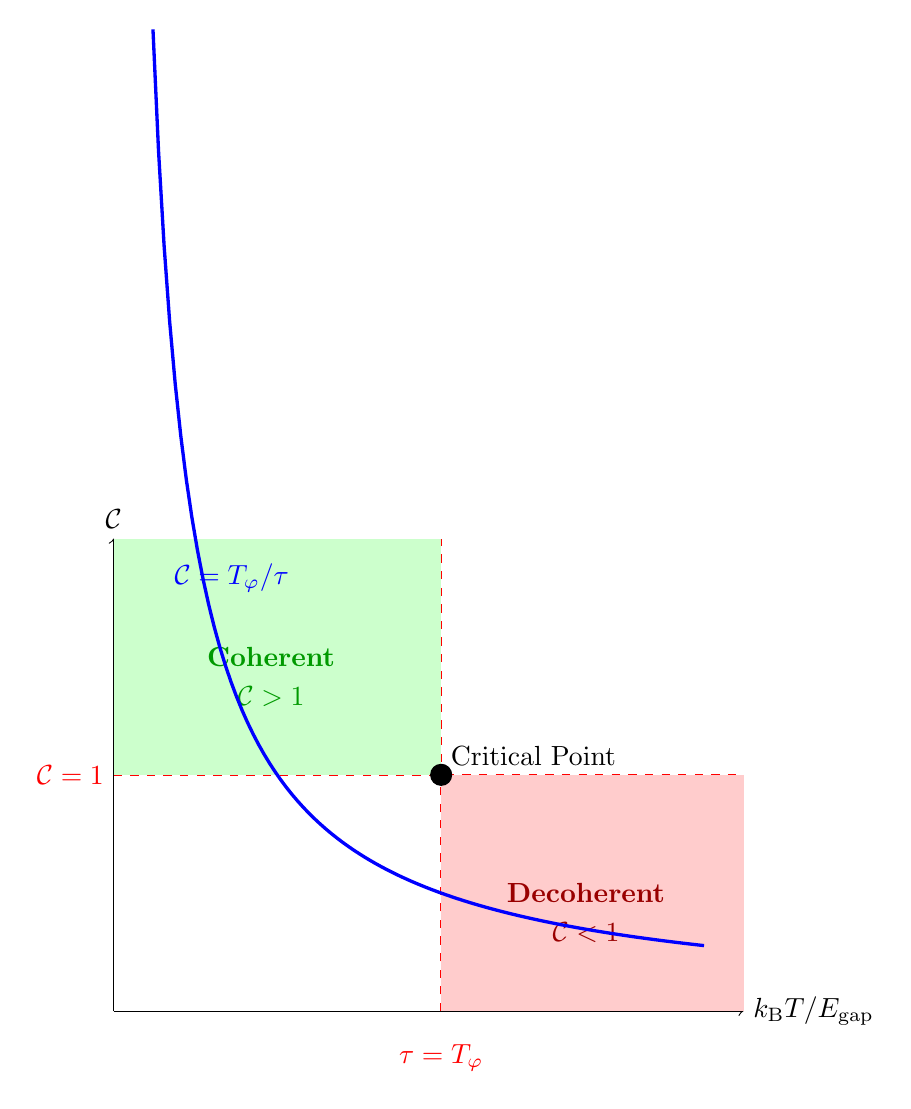
\begin{tikzpicture}[scale=1.0]
    % Axes
    \draw[->] (0,0) -- (8,0) node[right] {$\kB T / \Egap$};
    \draw[->] (0,0) -- (0,6) node[above] {$\Coh$};
    
    % Critical line
    \draw[red, thick, dashed] (0,3) -- (8,3);
    \node[red, left] at (0,3) {$\Coh = 1$};
    
    % Critical temperature
    \draw[red, thick, dashed] (4.16,0) -- (4.16,6);
    \node[red, below] at (4.16,-0.3) {$\tau = \Tphi$};
    
    % Coherent region
    \fill[green!20] (0,3) rectangle (4.16,6);
    \node[green!60!black] at (2,4.5) {\textbf{Coherent}};
    \node[green!60!black] at (2,4) {$\Coh > 1$};
    
    % Decoherent region
    \fill[red!20] (4.16,0) rectangle (8,3);
    \node[red!60!black] at (6,1.5) {\textbf{Decoherent}};
    \node[red!60!black] at (6,1) {$\Coh < 1$};
    
    % Hyperbolic curve C = T_phi / tau
    \draw[blue, very thick, domain=0.5:7.5, samples=100] 
        plot (\x, {2.078*3/\x});
    \node[blue] at (1.5,5.5) {$\Coh = \Tphi/\tau$};
    
    % Critical point
    \fill[black] (4.16,3) circle (4pt);
    \node[above right] at (4.16,3) {Critical Point};
\end{tikzpicture}
\end{center}

\subsection*{FIG. 2: Coherence Order Parameter vs Temperature}

\begin{center}
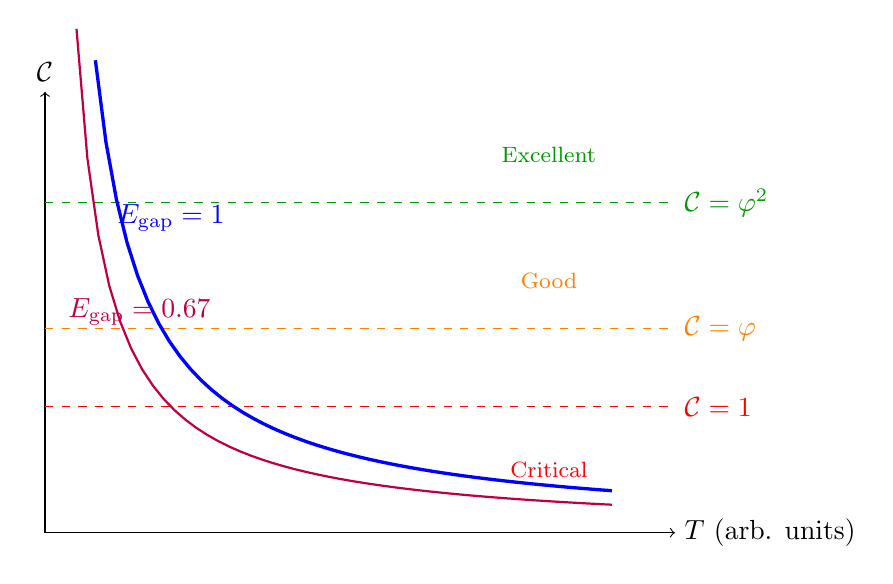
\begin{tikzpicture}[scale=0.8]
    % Axes
    \draw[->] (0,0) -- (10,0) node[right] {$T$ (arb. units)};
    \draw[->] (0,0) -- (0,7) node[above] {$\Coh$};
    
    % Threshold lines
    \draw[red, dashed] (0,2) -- (10,2) node[right] {$\Coh = 1$};
    \draw[orange, dashed] (0,3.24) -- (10,3.24) node[right] {$\Coh = \phival$};
    \draw[green!60!black, dashed] (0,5.24) -- (10,5.24) node[right] {$\Coh = \phival^2$};
    
    % Curves for different E_gap
    \draw[blue, very thick, domain=0.8:9, samples=50] 
        plot (\x, {6/\x});
    \node[blue] at (2,5) {$\Egap = 1$};
    
    \draw[purple, thick, domain=0.5:9, samples=50] 
        plot (\x, {4/\x});
    \node[purple] at (1.5,3.5) {$\Egap = 0.67$};
    
    % Zone labels
    \node[green!60!black] at (8,6) {\footnotesize Excellent};
    \node[orange] at (8,4) {\footnotesize Good};
    \node[red] at (8,1) {\footnotesize Critical};
\end{tikzpicture}
\end{center}

\subsection*{FIG. 3: Boltzmann Factor at Critical Temperature}

\begin{center}
\begin{tikzpicture}[scale=0.9]
    % Axes
    \draw[->] (0,0) -- (8,0) node[right] {$\tau = \kB T / \Egap$};
    \draw[->] (0,0) -- (0,5) node[above] {$\exp(-1/\tau)$};
    
    % Curve
    \draw[blue, very thick, domain=0.3:7, samples=100] 
        plot (\x, {4*exp(-1/\x)});
    
    % Golden ratio point
    \draw[red, dashed] (2.078,0) -- (2.078,2.47);
    \draw[red, dashed] (0,2.47) -- (2.078,2.47);
    \fill[red] (2.078,2.47) circle (4pt);
    
    \node[red, below] at (2.078,0) {$\Tphi$};
    \node[red, left] at (0,2.47) {$1/\phival$};
    
    % Annotations
    \node at (5,4) {$\exp(-1/\Tphi) = 1/\phival$};
    \draw[->] (5,3.7) -- (2.5,2.6);
\end{tikzpicture}
\end{center}

% ============================================================================
% END
% ============================================================================

\vfill
\begin{center}
\rule{0.5\textwidth}{0.5pt}\\[1em]
\textbf{END OF PATENT APPLICATION}
\end{center}

\end{document}

